\section{Auswertung}
\label{sec:Auswertung}

\subsection{Fehlerrechnung}
\label{sec:Fehlerrechnung}
Für die Fehlerrechnung werden folgende Formeln aus der Vorlesung verwendet.
für den Mittelwert gilt
\begin{equation}
    \overline{x}=\frac{1}{N}\sum_{i=1}^N x_i ß\; \;\text{mit der Anzahl N und den Messwerten x} 
    \label{eqn:Mittelwert}
\end{equation}
Der Fehler für den Mittelwert lässt sich gemäß
\begin{equation}
    \increment \overline{x}=\frac{1}{\sqrt{N}}\sqrt{\frac{1}{N-1}\sum_{i=1}^N(x_i-\overline{x})^2}
    \label{eqn:FehlerMittelwert}
\end{equation}
berechnen.
Wenn im weiteren Verlauf der Berechnung mit der fehlerhaften Größe gerechnet wird, kann der Fehler der folgenden Größe
mittels Gaußscher Fehlerfortpflanzung berechnet werden. Die Formel hierfür ist
\begin{equation}
    \increment f= \sqrt{\sum_{i=1}^N\left(\frac{\partial f}{\partial x_i}\right)^2\cdot(\increment x_i)^2}.
    \label{eqn:GaussMittelwert}
\end{equation}
 
\subsection{Inverting Amplifier}
\label{sec:InvertinAmpl}
 
Es wurden drei verschiedene Frequenzverhältnisse $\frac{R_2}{R_1}$ verwendet, zu welchen dann jeweils die Ausgangsamplituden in Abhängigkeit der Frequenz notiert wurden.
Die theoretischen Vergleichswerte für die Leerlaufverstärkung ergeben sich so zum
\begin{align*}
    V_{\text{1,t}} &= \frac{100\,\unit{\kilo\ohm}}{1\,\unit{\kilo\ohm}} =100\\
    V_{\text{2,t}} &= \frac{68\,\unit{\kilo\ohm}}{1\,\unit{\kilo\ohm}} =68\\
    V_{\text{1,t}} &= \frac{150\,\unit{\kilo\ohm}}{1\,\unit{\kilo\ohm}} =150\\
\end{align*}

Für das Verhältnisse ergeben sich folgende experimentell bestimmte Werte.
\begin{table}
    \centering
    \caption{Messwerte des Inverting Amplifiers mit $R1=1\,\unit{\kilo\ohm}$ und $R2=100\,\unit{\kilo\ohm}$}
    \begin{tabular}{c c c c}
        \toprule
        Frequenz $f\mathbin{/}\unit{\hertz}$ & Ausgangsampl. $U_0\mathbin{/}\unit{\volt}$& Eingangsampl. $U_{\text{i}}\mathbin{/}\unit{\volt}$ & Phasenverschiebung $\mathbin{/}$ rad\\
        \midrule
        5	&19.5	&0.21&	3.14\\
        30&	19.5	&0.21&	3.14\\
        60&	19.5	&0.21&	3.14\\
        120&	19.5&	0.21&	3.14\\
        240&	19.5&	0.21&	3.14\\
        480	&19.5	&0.21&	3.14\\
        960	&19.5	&0.21&	3.05\\
        1920&	19.2&	0.21&	2.97\\
        3840&	18.2&	0.21&	2.74\\
        7680&	14.9&	0.21&	2.34\\
        15280&	8.8&	0.21&	1.83\\
        30480&	5.1	&0.23& 1.71\\
        60000&	2.9	&0.23&	1.61\\
        120000&	1.6	&0.23&	1.43\\
        240000&	1.2	&0.23&	1.22\\
        \bottomrule
    \end{tabular}
    \label{tab:InvAmp1}
\end{table}

\begin{table}
    \centering
    \caption{Messwerte des Inverting Amplifiers mit $R1=1\,\unit{\kilo\ohm}$ und $R2=68\,\unit{\kilo\ohm}$}
    \begin{tabular}{c c c c}
        \toprule
        Frequenz $f\mathbin{/}\unit{\hertz}$ & Ausgangsampl. $U_0\mathbin{/}\unit{\volt}$& Eingangsampl. $U_{\text{i}}\mathbin{/}\unit{\volt}$ & Phasenverschiebung $\mathbin{/}$ rad\\
        \midrule
        15&	27.0&	0.44&	3.14\\		    
        30&	27.0&	0.44&	3.12\\		
        60&	27.0&	0.44&	3.12\\		
        120&	27.0&	0.44&	3.09\\		
        240&	27.0&	0.44&	3.09\\		
        480	&27.0&	0.44&	3.09\\		
        960	&27.0&	0.44&	3.07\\		
        1900&	26.6&	0.44&	3.00\\	
        3800& 26.3&	0.44&	2.83\\	
        7700&	20.5&	0.44&	2.25\\	
        15000&	10.8&	0.44&	1.73\\	
        30000&	5.3&	0.44&	1.41	\\	
        60000&	3.1	&0.44&	1.31	\\	
        120000&	1.7	&0.44&	1.22	\\	
        240000&	1.3	&0.44&	1.13	\\
        \bottomrule
    \end{tabular}
    \label{tab:InvAmp2}
\end{table}


\begin{table}
    \centering
    \caption{Messwerte des Inverting Amplifiers mit $R1=1\,\unit{\kilo\ohm}$ und $R2=150\,\unit{\kilo\ohm}$}
    \begin{tabular}{c c c c}
        \toprule
        Frequenz $f\mathbin{/}\unit{\hertz}$ & Ausgangsampl. $U_0\mathbin{/}\unit{\volt}$& Eingangsampl. $U_{\text{i}}\mathbin{/}\unit{\volt}$ & Phasenverschiebung $\mathbin{/}$ rad\\
        \midrule
        15& 27.0&	320&	3.16\\		
        30&	27.0&	320&	3.14\\		
        60&	27.0&	320&	3.14\\		
        120&	27.0&	320&	3.14\\		
        240&	27.0&	320&	3.14\\		
        480&	26.8&	320&	3.05\\		
        960&	26.5&	320&	3.02\\		
        1900&	26.5&	320&	2.84\\	
        3800&	24.2&	320&	2.58\\	
        7700&	16.0&	320&	1.95\\	
        15000&	9.5&	320&	1.78\\		
        30000&	5.2&	320&	1.68\\		
        60000&	3.0&	320&	1.43\\	
        120000&	1.8&	320&	1.26\\	
        240000&	1.4&	320& 1.08	\\
        \bottomrule
    \end{tabular}
    \label{tab:InvAmp3}
\end{table}

\newpage

\subsection{Integrator}
\begin{table}
    \centering
    \caption{Messwerte des Integrators mit $R=10\,\unit{\kilo\ohm}$ und $C=100\,\unit{\nano\farad}$}
    \begin{tabular}{c c c}
        \toprule
        Frequenz $f\mathbin{/}\unit{\hertz}$ & Eingangsspannung $U_{\text{E}}\mathbin{/}\unit{\volt}$& Ausgangsspannung $U_{\text{A}}\mathbin{/}\unit{\volt}$ \\
        \midrule
        7& 3.02 & 28.6 \\
        15 & 3.02 & 26.1 \\
        20 & 3.02 & 20.6 \\
        30 & 3.02 & 15.0 \\
        45 & 3.02 & 10.8 \\
        60 & 3.02 & 8.5 \\
        90 & 3.02 & 6.2 \\
        120 & 3.02 & 4.7 \\
        180 & 3.02 & 3.5 \\
        240 & 3.02 & 2.8 \\
        350 & 3.02 & 2.3 \\
        480 & 3.02 & 1.7 \\
        700 & 3.02 & 1.5 \\
        960 & 3.02 & 1.4 \\
        \bottomrule
    \end{tabular}
    \label{tab:Integrator}
\end{table}

um: -0.738+/-0.021 ub: 4.07+/-0.10

\begin{figure}
    \centering
    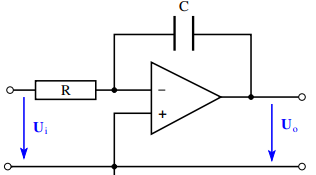
\includegraphics[width=0.8\textwidth]{build/integrator.pdf}
    \caption{Verstärkung $U_A/U_E$ eines Integrators in Abhängigkeit von der Frequenz.}
    \label{fig:intplot}
\end{figure}

\subsection{Differentiator}
\begin{table}
    \centering
    \caption{Messwerte des Differentiators mit $R=100\,\unit{\kilo\ohm}$ und $C=22\,\unit{\nano\farad}$}
    \begin{tabular}{c c c}
        \toprule
        Frequenz $f\mathbin{/}\unit{\hertz}$ & Eingangsspannung $U_{\text{E}}\mathbin{/}\unit{\volt}$& Ausgangsspannung $U_{\text{A}}\mathbin{/}\unit{\volt}$ \\
        \midrule
        7& 6.15 & 1.1 \\
        15 & 5.99 & 1.6 \\
        20 & 5.99 & 2.1 \\
        30 & 5.99 & 2.9 \\
        45 & 6.15 & 3.9 \\
        60 & 5.99 & 5.3 \\
        90 & 5.99 & 7.8 \\
        120 & 5.99 & 11.5 \\
        180 & 5.99 & 14.3 \\
        240 & 5.99 & 19.1 \\
        350 & 5.99 & 27.1 \\
        \bottomrule
    \end{tabular}
    \label{tab:Differentiator}
\end{table}

um: 0.869+/-0.023 ub: -3.63+/-0.10

\begin{figure}
    \centering
    \includegraphics[width=0.8\textwidth]{build/differentiator.pdf}
    \caption{Verstärkung $U_A/U_E$ eines Differentiators in Abhängigkeit von der Frequenz.}
    \label{fig:diffplot}
\end{figure}


\subsection{Generator mit variierender Amplitude}
\begin{figure}
    \centering
    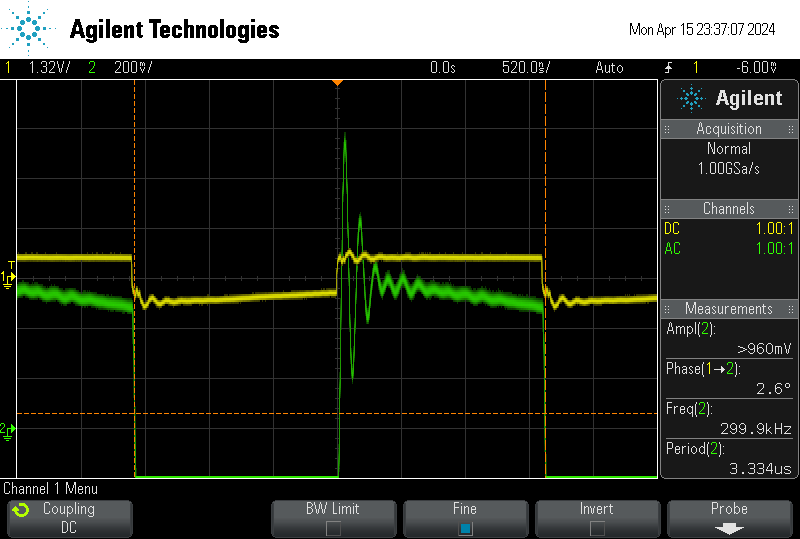
\includegraphics[width=0.7\textwidth]{genvarplot.png}
    \caption{Verlauf der gedämpften Oszillation.}
    \label{fig:genvarosz}
\end{figure}

\begin{figure}
    \centering
    \includegraphics[width=0.8\textwidth]{build/genvar.pdf}
    \caption{Verlauf der Amplituden der gedämpften Oszillation}
    \label{fig:genvarAmo}
\end{figure}